\documentclass{article}
\usepackage{tikz}
\usetikzlibrary{shapes.multipart, positioning, arrows.meta}

\begin{document}
\begin{figure}[htbp]
\centering
\vspace{1cm}
\resizebox{\textwidth}{!}{
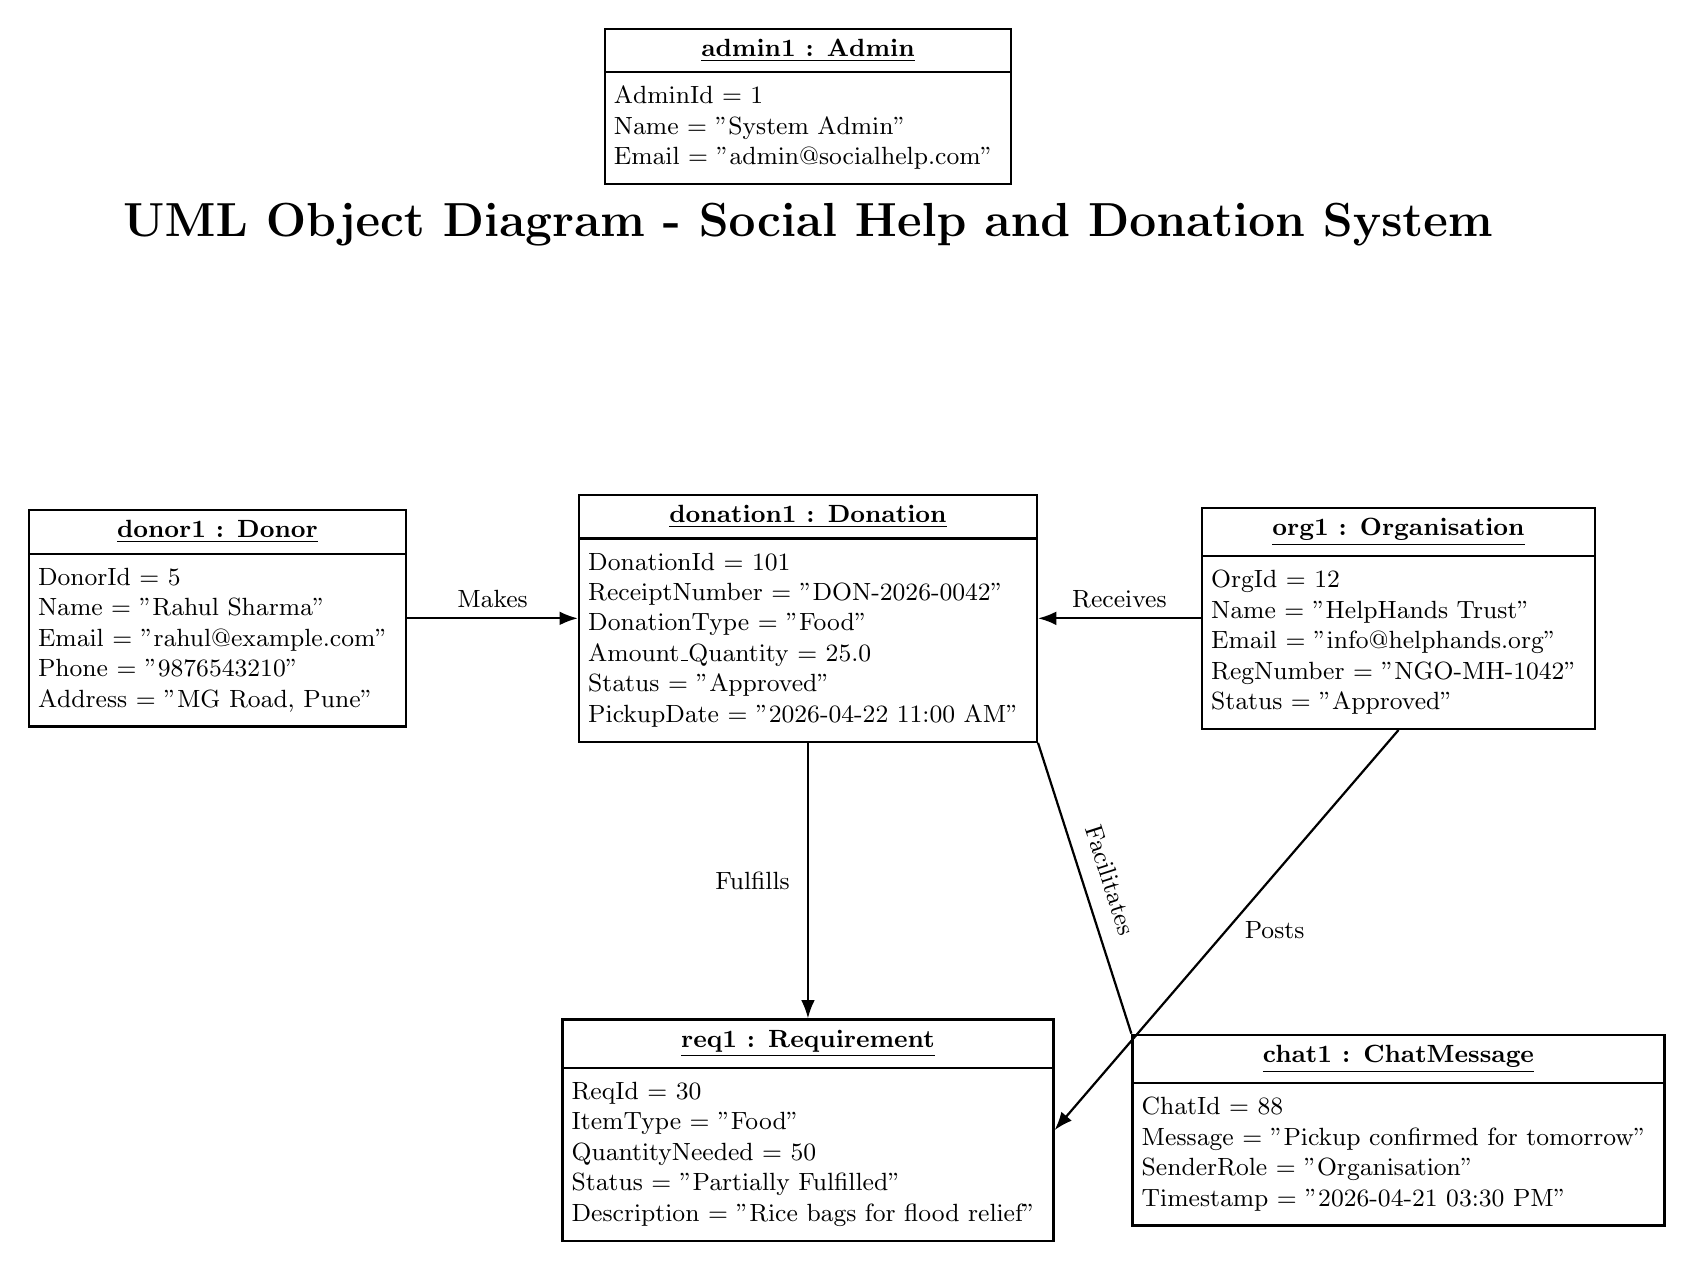
\begin{tikzpicture}[
    >=Latex,
    object/.style={
        draw, rectangle split, rectangle split parts=2,
        minimum width=4cm, align=center, fill=white, thick, font=\small
    }
]

% Title
\node[font=\LARGE\bfseries, align=center] at (0, 5) {UML Object Diagram - Social Help and Donation System};

% -------------------------
% Object Instances Definition
% -------------------------

% 1. Donation (Center)
\node[object] (donation1) at (0, 0) {
    \underline{\textbf{donation1 : Donation}}
    \nodepart{second}
    \normalfont
    \begin{tabular}{@{}l@{}}
    DonationId = 101 \\
    ReceiptNumber = "DON-2026-0042" \\
    DonationType = "Food" \\
    Amount\_Quantity = 25.0 \\
    Status = "Approved" \\
    PickupDate = "2026-04-22 11:00 AM"
    \end{tabular}
};

% 2. Donor (Left)
\node[object] (donor1) at (-7.5, 0) {
    \underline{\textbf{donor1 : Donor}}
    \nodepart{second}
    \normalfont
    \begin{tabular}{@{}l@{}}
    DonorId = 5 \\
    Name = "Rahul Sharma" \\
    Email = "rahul@example.com" \\
    Phone = "9876543210" \\
    Address = "MG Road, Pune"
    \end{tabular}
};

% 3. Organisation (Right)
\node[object] (org1) at (7.5, 0) {
    \underline{\textbf{org1 : Organisation}}
    \nodepart{second}
    \normalfont
    \begin{tabular}{@{}l@{}}
    OrgId = 12 \\
    Name = "HelpHands Trust" \\
    Email = "info@helphands.org" \\
    RegNumber = "NGO-MH-1042" \\
    Status = "Approved"
    \end{tabular}
};

% 4. Requirement (Bottom Center)
\node[object] (req1) at (0, -6.5) {
    \underline{\textbf{req1 : Requirement}}
    \nodepart{second}
    \normalfont
    \begin{tabular}{@{}l@{}}
    ReqId = 30 \\
    ItemType = "Food" \\
    QuantityNeeded = 50 \\
    Status = "Partially Fulfilled" \\
    Description = "Rice bags for flood relief"
    \end{tabular}
};

% 5. Admin (Top Center)
\node[object] (admin1) at (0, 6.5) {
    \underline{\textbf{admin1 : Admin}}
    \nodepart{second}
    \normalfont
    \begin{tabular}{@{}l@{}}
    AdminId = 1 \\
    Name = "System Admin" \\
    Email = "admin@socialhelp.com"
    \end{tabular}
};

% 6. ChatMessage (Bottom Right)
\node[object] (chat1) at (7.5, -6.5) {
    \underline{\textbf{chat1 : ChatMessage}}
    \nodepart{second}
    \normalfont
    \begin{tabular}{@{}l@{}}
    ChatId = 88 \\
    Message = "Pickup confirmed for tomorrow" \\
    SenderRole = "Organisation" \\
    Timestamp = "2026-04-21 03:30 PM"
    \end{tabular}
};

% -------------------------
% Path Connections (Specific Instance Links)
% No multiplicities in Object Diagrams!
% -------------------------

% donor1 -> donation1
\draw[->, thick] (donor1.east) -- (donation1.west) 
    node[midway, above, font=\small] {Makes};

% org1 -> donation1
\draw[->, thick] (org1.west) -- (donation1.east) 
    node[midway, above, font=\small] {Receives};

% org1 -> req1
\draw[->, thick] (org1.south) -- (req1.east) 
    node[midway, right=0.1cm, font=\small] {Posts};

% donation1 -> req1
\draw[->, thick] (donation1.south) -- (req1.north) 
    node[midway, left=0.1cm, font=\small] {Fulfills};

% donation1 -> chat1
\draw[-, thick] (donation1.south east) -- (chat1.north west) 
    node[midway, above=0.1cm, font=\small, sloped] {Facilitates};

\end{tikzpicture}
}
\end{figure}
\end{document}
